\documentclass[12pt]{beamer}

\author{ 李小飞}
\title{\textbf{工~程~数~学}}
\subtitle{Engineering Mathematics}
\institute[电子科技大学]{{\large 光电科学与工程学院}}
\date[] {Very Good Lecture ,  Sept. 2021}
\logo{
\includegraphics[height=1cm]{uestclogo}}
\usepackage{mybeamer}

\begin{document}      
%%%%%%%%%%%%%%%%%%%%%%%%%%%%%%%%%
\begin{frame}[plain]
	%\maketitle
	\titlepage
\end{frame}

%%%%%%%%%%%%%%%%%%%%%%%%%%%%%%%%%
% 目录
\begin{frame}[allowframebreaks]
	\tableofcontents
	% You might wish to add the option [pausesections]
\end{frame}

%%%%%%%%%%%%%%%%%%%%%%%%%%%%%%%%%%%%%%%%%%%%%%%%%
\section{主题一}


\begin{frame}
	\frametitle{标题}	
	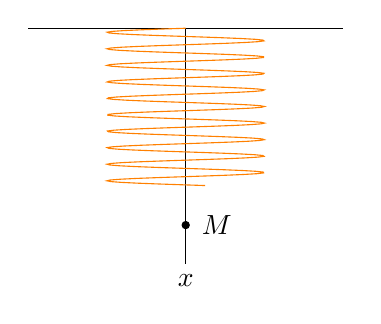
\begin{tikzpicture}
			\draw  (-2,0) -- (2,0) node[below] {};
			\draw  (0,0) -- (0,-3) node[below] {$x$};	
			\draw [orange, domain=0:-2, samples=200] plot({sin(\x r *30},\x);
			\draw [fill, black, circle] (0,-2.5) circle(0.3ex) node[right] {$M$};
  \end{tikzpicture} 
	
\end{frame}

%%%%%%%%%%%%%%%%%%%%%%%%%%%%%%%%%%%%%%%%%%%%%%%%%
\section{主题二}

\begin{frame}
\frametitle{区块}
	\begin{block}{勾X定理}
		直角三角形的斜边的平方等于两直角边的平方和。
		可以用符号语言表述为:设直角三角形ABC,其中$\angle C=90^\circ \int_{0}^{\infty}$则有
		\begin{equation}
			AB^2=BC^2+AC^2 \int
		\end{equation}
	\end{block}

\end{frame}


\begin{frame}
	\begin{itemize}
		\item test
		\item test
	\end{itemize}

\end{frame}

%%%%%%%%%%%%%%%%%%%%%%%%%%%%%%%%%%%%%%%%%%%%%%%%%
\section{主题三}

\begin{frame}
	\frametitle{标题}	
	
\end{frame}

\begin{frame}
	\frametitle{Sample frame title}
	
	In this slide, some important text will be
	\alert{highlighted} because it's important.
	Please, don't abuse it.
	
	\begin{block}{Remark}
		Sample text
	\end{block}
	
	\begin{alertblock}{Important theorem}
		Sample text in red box
	\end{alertblock}
	
	\begin{examples}
		Sample text in green box. The title of the block is ``Examples".
	\end{examples}
\end{frame}

\begin{frame}
	\frametitle{Sample frame title}
	This is a text in second frame. 
	For the sake of showing an example.
	
	\begin{itemize}
		\item<1-> Text visible on slide 1
		\item<2-> Text visible on slide 2
		\item<3> Text visible on slide 3
		\item<4-> Text visible on slide 4
	\end{itemize}
\end{frame}



%%%%%%%%%%%%%%%%%%%%%%%%%%%%%%%%%%%%%%%%%%%%%%%%%
\begin{frame}
	\begin{center}
		\huge Thanks for your attention! \\ Q \& A
	\end{center}
\end{frame}

%%%%%%%%%%%%%%%%%%%%%%%%%%%%%%%%%%%%%%%%%%%%%%%%%
\end{document}